\section{Setting up the Beowulf Cluster}
\label{beowulf_setup}
\subsection{Cluster components}
Computer cluster is made up of various hardware and software components with complex interactions between different components. Figure \ref{fig:cluster-layers} depicts the various components that form a cluster.

\begin{figure}[!htb]
 \center
  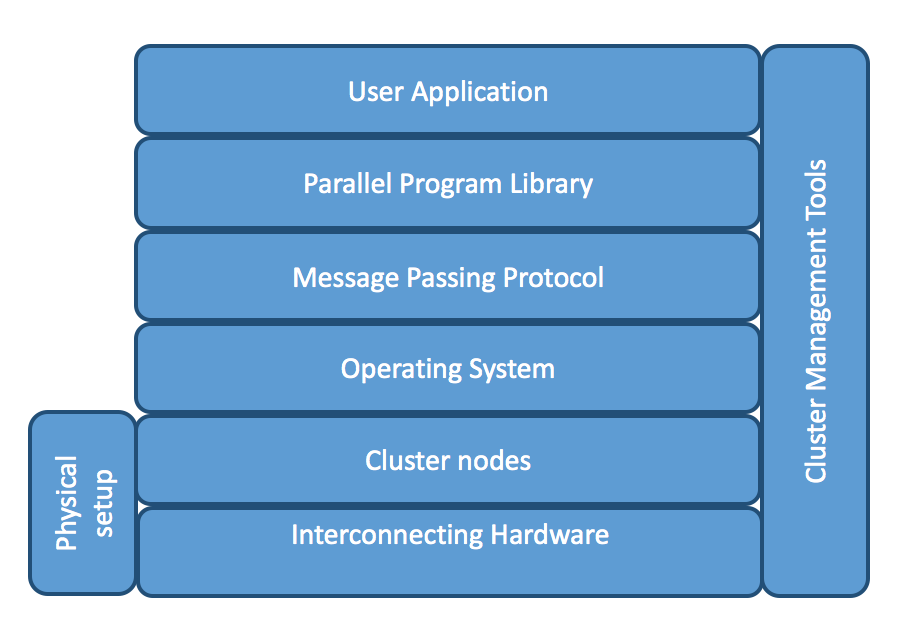
\includegraphics[width= .75 \linewidth]{figs/cluster/cluster_layers.png}
  \caption{Layers in a Cluster}
  \label{fig:cluster-layers}
   \center
\end{figure}

A Beowulf cluster contains a set of cluster nodes. A node can be a server with a specific role within the cluster or it can be a compute node. All of the nodes are connected using a dedicated Local Area Network(LAN) or System Area Network(SAN). The complexity of networking topology is depends on directly to number of nodes in the cluster.

As shown in Figure \ref{fig:cluster-layers} to setup a cluster we need following hardware and software components:

\paragraph{Cluster Nodes}
Cluster nodes are stand-alone computers with one or more CPUs, own Memory unit, and Network Interface Card(NIC). A node may contain it's own local secondary storage or could be configured as disk-less workstation. For this implementation nodes were configured with their own local storage to reduce network overhead for accessing boot-image and runtime libraries during boot up and program execution. However, Network File Sharing(NFS) was implemented to streamline program execution environments across the Cluster. The details of nodes configurations are discussed later in this chapter for both virtual and physical implementation.

\paragraph{Interconnecting Hardware}
This is networking components of the cluster that facilitates nodes communicating with one another. Since communication is the key part of cluster computing this is very important component that can define the overall performance. For this project a simple ethernet network was configured for both virtual and physical implementation. For the physical setup, Thompson Broadband Router (Model: TWG870) was used. This router has 4 Gigabit ports that facilitated to setup a Gigabit LAN for the cluster-only network.

\paragraph{Operating System}
Linux is widely used on Beowulf cluster because of its hardware support, performance, its free and open source kernel. For this project Ubuntu Server 16.04 was chosen.

\paragraph {Message Passing Protocol}
There are two typical approaches to communication between cluster nodes, one is  Parallel Virtual Machine(PVM) and the other is Message Passing Interface (MPI). However, MPI has now emerged as the de facto standard for message passing on computer clusters. The objective of this project is parallelising SGA using MPI libraries therefore, MPI was chosen message passing protocol for obvious reason.

\paragraph {Parallel Program Library}
MPI has many implementation. There are two free and popular MPI libraries available, one is OpenMPI and another is MPICH. For this project MPICH 3.2 is installed on each nodes. 

\paragraph {Cluster management tools}

\subsection{Topological design}
Figure \ref{fig:beowulf-cluster} shows a simple Beowulf cluster setup that was adopted for this project implementation. For simplicity the implemented Beowulf contains a Master node and 3 to 4 compute nodes which is extendable.

\begin{figure}[!htb]
  \includegraphics[width=\linewidth]{figs/cluster/beowulf_cluster.png}
  \caption{A typical Beowulf setup}
  \label{fig:beowulf-cluster}
\end{figure}

Beowulf cluster was simulated in virtual environment using Oracle VirtualBox and then actual hardware implementation was done using commodity physical hardware. In both cases the software suits and configuration was identical with minor changes.

\subsection{Virtual nodes}
Table \ref{tab:virt_node_conf} shows the node configuration when using simulated hardware using VirtualBox on Macbook Pro(2.6GHz Intel core i5, 16 GB RAM, 256GB SSD) host computer.

%% Node description table 
\begin{table}[!htb]
\centering
\caption{Virtual nodes configuration}
\begin{tabular}{|l|l|l|l|}
\hline
Hostname & Role & IPv4 address & Hardware Config \\ \hline
master & Master & 192.168.56.10/24 & Single core, 2GB RAM, 10 GB HDD \\ \hline
node1 & Slave & 192.168.56.11/24 & Single core, 2GB RAM, 10 GB HDD \\ \hline
\end{tabular}
\label{tab:virt_node_conf}
\end{table}

\subsection{Physical nodes}
Table \ref{tab:phy_node_conf} shows the node configuration of using physical components. 
%% Physicle node description table 
\begin{table}[!htb]
\centering
\caption{Physical nodes configuration}
\begin{tabular}{|l|l|l|l|}
\hline
Hostname & Role & IPv4 address & Hardware Config \\ \hline
padma & Master & 172.16.0.1/24 & Dell Dual-core, 6GB RAM, 160 GB HDD \\ \hline
meghna & Slave & 172.16.0.15/24 & HP Dual-core, 2GB RAM, 160 GB HDD \\ \hline
jamuna & Slave node & 172.16.0.17/24 & HP Dual-core, 2GB RAM, 160 GB HDD \\ \hline
\end{tabular}
\label{tab:phy_node_conf}
\end{table}

\afterpage{\clearpage}

\subsection{Setup \& Configuration}
\subsubsection{Setup steps}
\begin{itemize}
	\item Install Operating Systems(OS) for each nodes
	\item Configure network settings
	\item Create MPI user
	\item Configure Network File Share
	\item Configure SSH password-less login
	\item Install MPI libraries, compiler and build tools
	\item Administrative tasks
\end{itemize}

\subsubsection{Installing Operating System} 
Popular Linux distribution Ubuntu Server 16.04 was chosen as OS for all cluster nodes. It was installed with default settings and without any GUI or window manager. A desktop environment was not needed as it would have reduced the performance of our Beowulf system. Therefore our installation of Ubuntu Linux was a minimal system and OpenSSH server.

After a successful installation of the operating system, we needed to set up the network and, of course, the shared file system for the compute nodes. For the shared file system, we installed the NFS server on the first node, which operates as the head node. Then, we exported the locations for the shared file system from there.

\subsubsection{Network configuration - Master node}

Identify network interface card and its name
\begin{lstlisting}[style=BashInputStyle]
$ip link show
\end{lstlisting}

And from the output shown as below we identify the NIC names that we want to configure in following steps

%\begin{lstlisting}[style=BashInputStyle, caption={Network device configuration file}, label={lst:config_net_dev}]
\begin{lstlisting}[style=BashInputStyle]
1: lo: <LOOPBACK,UP,LOWER_UP> mtu 65536 qdisc noqueue state UNKNOWN mode DEFAULT group default qlen 1
    link/loopback 00:00:00:00:00:00 brd 00:00:00:00:00:00
2: enp2s0: <BROADCAST,MULTICAST,UP,LOWER_UP> mtu 1500 qdisc pfifo_fast state UP mode DEFAULT group default qlen 1000
    link/ether ec:08:6b:04:62:df brd ff:ff:ff:ff:ff:ff
3: enp0s25: <BROADCAST,MULTICAST,UP,LOWER_UP> mtu 1500 qdisc pfifo_fast state UP mode DEFAULT group default qlen 1000
    link/ether 00:19:d1:73:38:60 brd ff:ff:ff:ff:ff:ff
\end{lstlisting}

To configure the network configuration file /etc/network/interfaces need to be edited as follows:
\begin{lstlisting}[style=BashInputStyle]
auto lo
iface lo intet loopback

# The primary network interface(connected to public network)
auto enp0s25
iface enp0s25 intet static
	address 192.168.0.14
	netmask 255.255.255.0
	gateway 192.168.0.1
	dns-nameserver 89.101.160.5  8.8.8.8

# The cluster network interface
auto enp2s0
iface enp2s0 intet static
	address 172.16.0.1
	netmask 255.255.255.0
\end{lstlisting}

System's host file( /etc/hosts ) needs to be edited for each node for easier host look up.

\begin{lstlisting}[style=BashInputStyle]	
127.0.0.1	localhost
172.16.0.1	padma
172.16.0.2	meghna
172.16.0.3	jamuna
\end{lstlisting}

Then scp this file to other nodes and copy it with privileged user into /etc directory.

\begin{lstlisting}[style=BashInputStyle]
	$scp /etc/hosts meghna:~/
	$ssh meghna
	$sudo cp hosts /etc/hosts
	$scp /etc/hosts jamuna:~/
	$ssh jamuna
	$sudo cp hosts /etc/hosts
\end{lstlisting}

\subsubsection{Create MPI user}
Create a user for running MPI jobs. This user needs to created with same user ID and group ID on each node.

\begin{lstlisting}[style=BashInputStyle]
	$sudo adduser mpiuser --uid 999
\end{lstlisting}

\subsubsection{Network File System configuration}

Install and setup the Network File System
\begin{lstlisting}[style=BashInputStyle]
# Master node
padma$ sudo apt-get install nfs-kernel-server
padma$ sudo apt-get install nfs-common
# And compute nodes
meghna$ sudo apt-get install nfs-common
jamuna$ sudo apt-get install nfs-common
\end{lstlisting}

Next we need to share mpiuser home directory with all other nodes. To do this the file /etc/exports on the master node needs to be edited to add the share directory.

\begin{lstlisting}[style=BashInputStyle]
	/home/mpiuser 172.16.0.0/24(rw,sync,no_subtree_check)
\end{lstlisting}


At this point NFS server needs to be restarted to make share directory available across the network.

\begin{lstlisting}[style=BashInputStyle]
master:~\$ sudo service nfs-kernel-server restart
sudo exportfs -a
\end{lstlisting}

Now we can check and confirm from compute node if the NFS shared directory can be mount.

\begin{lstlisting}[style=BashInputStyle]
	showmount -e padma
\end{lstlisting}

This should show the export list from master node as below:
\begin{lstlisting}[style=BashInputStyle]
Export list for padma:
/home/mpiuser 172.16.0.0/24
\end{lstlisting}

To mount this shared directory from other nodes we can execute the command below from the shell.

\begin{lstlisting}[style=BashInputStyle]
meghna:~\$ sudo mount master:/home/mpiuser /home/mpiuser
jamuna:~\$ sudo mount master:/home/mpiuser /home/mpiuser
\end{lstlisting}

And to mount the share directory at system boot up without having to enter the command manually, the following entry is added to all compute nodes in the file /etc/fstab.

\begin{lstlisting}[style=BashInputStyle]
	padma:/home/mpiuser /home/mpiuser nfs
\end{lstlisting}

\subsubsection{Configure password less communication}
All MPI nodes should be able to communicate with other nodes without having to provide any password. This is achieved by configuring password-less SSH between nodes.

If ssh is not installed with during the OS installation steps we could install it by running the following command on each nodes:
\begin{lstlisting}[style=BashInputStyle]
	$sudo apt-get install ssh
\end{lstlisting}

Next step is to generate a SSH key for  'mpiuser' on all nodes. The SSH key is by default created in the user's home directory. In our case the 'mpiuser' home directory  which is located at /home/mpiuser. This is actually the same directory for all nodes i.e  /home/mpiuser on the master node since the home directory is a NFS mount. So, the SSH key for the 'mpiuser' was generated on master node, and all other nodes will automatically have an SSH key in 'mpiuser' home directory. 

To generate an SSH key for the MPI user on the master node (but any node should be fine).
\begin{lstlisting}[style=BashInputStyle]
	\$ su mpiuser
	\$ ssh-keygen
\end{lstlisting}

When asked for a passphrase, this needs to be left empty (hence password-less SSH).

When done, the 'mpiuser' should have same ssh-key on its home directory which is accessible from all nodes in the cluster. Now, the master node needs to be able to automatically login to the compute nodes. To enable this, the public SSH key of the master node needs to be added to the list of known hosts (this is usually a file \~/.ssh/authorized\_keys) of all compute nodes. All SSH key data is stored in one location: /home/mpiuser/.ssh/ on the master node. So instead of having to copy master node's public SSH key to all compute nodes separately, we just have to copy it to master's own authorized\_keys file. There is a command to push the public SSH key of the currently logged in user to another computer. To do that we run the following commands on the master node as user "mpiuser",
\begin{lstlisting}[style=BashInputStyle]
	mpiuser@master:~\$ ssh-copy-id localhost
\end{lstlisting}

Master node's own public SSH key should now be copied to /home/mpiuser/.ssh/authorized\_keys. But since /home/mpiuser/ (and everything under it) is shared with all nodes via NFS, all nodes should now have master's public SSH key in the list of known hosts. This means that we should now be able to login on the compute nodes from the master node securely without having to enter a password,

\begin{lstlisting}[style=BashInputStyle]
	mpiuser@master:~$ ssh meghna
	mpiuser@meghna:~$ echo $HOSTNAME
	meghna
\end{lstlisting}

The user 'mpiuser' should be now be able to login on node1 via SSH. At this stage login to other nodes also be checked.

\subsubsection{Install MPI libraries, compiler and build tools}
On each node we needed to install C/C++ libraries and headers files along with required build tools. After that we installed MPICH 3.2 version of MPI library using Ubuntu's default source repository.

\begin{lstlisting}[style=BashInputStyle]
	$sudo apt-get install build-essential
	$sudo apt-get install mpich
	$mpicc -v  \# To check MPICH version OR
	$mpiexec --version
\end{lstlisting}

\subsubsection{Configuring MPI Process Manager}
\label{beowulf:process_manager}
A process manager is needed for MPI programs are to spawn and manage parallel cluster. This process manager is an external entity. In MPICH implementation of MPI library these process managers communicate with MPI processes using a predefined interface called as PMI (Process Management Interface). The process manager included with MPICH 3.2 installation is called Hydra.
In order to setup Hydra, we need to create one file on the master node. This file contains all the host names of the compute nodes. This file can be put in anywhere, but for simplicity it is created in the the MPI user?s home directory. This file only needs to be present on the node that will be used to start jobs on the cluster, usually the master node. Hydra uses this file to spawn process in the cluster in round robin manner. Since the MPI home directory is shared among all nodes, all nodes will have the hosts file. This file is created using following command where the file is named \textit{hosts}:

\begin{lstlisting}[style=BashInputStyle]
	$cd ~
	$touch hosts
\end{lstlisting}

For this Beowulf setup the following entries are added to this \textit{hosts} file: 
\begin{lstlisting}[style=BashInputStyle]
padma:2
meghna:2
jamuna:2
\end{lstlisting}


